\documentclass[toc=sectionentrywithdots,a4paper,11pt,oneside, openright]{scrartcl}

% Stilistische Vorgaben nach Standard der HS
%--------------------------------------------------------------------------
\usepackage{geometry}
\geometry{top=2.0cm,bottom=3cm,left=3.5cm,right=2cm}
%----------------Schriftart/-form------------------
%Serifen######
%-------------
%\usepackage{mathptmx} % setzt auf Times New Roman
%\renewcommand{\familydefault}{\rmdefault}
\setkomafont{section}{\fontfamily{\rmdefault}\Large}
\setkomafont{subsection}{\fontfamily{\rmdefault}\large}
\setkomafont{subsubsection}{\fontfamily{\rmdefault}\normalsize}
\setkomafont{sectionentry}{\fontfamily{\rmdefault}}

%Seriflos#####
%-------------
\renewcommand{\familydefault}{\sfdefault}
%\setkomafont{section}{\fontfamily{\sfdefault}\Large}
%\setkomafont{subsection}{\fontfamily{\sfdefault}\large}
%\setkomafont{subsubsection}{\fontfamily{\sfdefault}\normalsize}
%\setkomafont{sectionentry}{\fontfamily{\sfdefault}}
%---------------------------------------------------
\usepackage[T1]{fontenc} %
\usepackage{setspace}
\setcounter{tocdepth}{4}
%--------------------------------------------------------------------------
% Pakete für die Bearbeitung (Sprache, Tabellen, Grafiken, Mathe,...)
\usepackage[ngerman]{babel} % Sprachpaket
\usepackage[utf8]{inputenc} % Zeichenkodierung inkl. Umlaute
\usepackage{graphicx} % Einbinden von Bildern
\usepackage{longtable} % Tabellen die über eine Seite gehen
\usepackage{tabularx} % Standardtabellen
\usepackage{amsmath} % Für mathematische Zeichen, Formeln, etc...
\usepackage{tabto}
\usepackage{blindtext}
%Abkürzungsverzeichnis; Option: acronym trägt nur die Abkürzungen in das Verzeichnis ein. Kompilieren im TeXStudio über Tools-->Glossary-->dann gesamtest Dokument kompilieren
\usepackage[nonumberlist,nomain,acronym,xindy,automake,toc]{glossaries}
\makeglossaries
\loadglsentries{_glossary.tex}

%Kopf-/Fußzeile
%------------
\usepackage{fancyhdr}
\pagestyle{fancy}
\fancypagestyle{plain}{\fancyhf{}}
\fancyhf{}
\rfoot{\thepage}
\renewcommand{\headrulewidth}{0pt}
\renewcommand{\footrulewidth}{0pt}
%--------------------------------------------------------------------------
\usepackage[backend=biber,sorting=none]{biblatex}
\addbibresource{_bibliography.bib}

%-------------------------------------
% eigene pakete
\usepackage{textcomp}
\usepackage{graphicx}
\usepackage{float}
\usepackage{enumitem}
\usepackage{csquotes}
\usepackage[breaklinks]{hyperref}

%---------------------------------------------------
% PLATZHALTER FÜLLEN MIT NAMEN, THEMA, ETC.
\newcommand{\grad}{Bachelor of Science}
\newcommand{\matrinr}{s158109}
\newcommand{\thema}{Untersuchung des Einsatzes der Blockchain-Technologie bei Smart Locks anhand eines Prototypen hinsichtlich der Sicherheit}
\newcommand{\name}{Janine Kostka}
\newcommand{\geb}{08.01.1994}
\newcommand{\ort}{Kirchheim unter Teck}
\newcommand{\erstp}{Prof. Dr. rer.pol.habil. Benjamin Fabian}
\newcommand{\instituterst}{Hochschule für Telekommunikation Leipzig}
\newcommand{\zweitp}{M.Eng. Mario Hoffmann}
\newcommand{\institutzweit}{Hochschule für Telekommunikation Leipzig}
\newcommand{\abgabe}{31.10.2018}
%---------------------------------------------------


\begin{document}
	%---------------------------------------------------
	% TITELSEITE/DECKBLATT
	\begin{titlepage}
		\begin{figure}[h]
			
\includegraphics[scale=0.2]{hftl_logo.png}
		\end{figure}
		\vspace*{20pt}
		\centering
		Hochschule für Telekommunikation Leipzig\\
		\vspace*{40pt}
		\large \textbf{Abschlussarbeit zur Erlangung des akademischen Grades}\\
		\doublespacing
		\textbf{\grad} % ggf. Grad anpassen
		\vspace*{100pt}
		\begin{table}[h!]
			\begin{tabular}{p{0.2\linewidth}p{0.7\linewidth}}
				Thema: & \large \thema \\
				\\[4em]
				\\[5em]
				Vorgelegt von: & \large \name  \\
				\\[2em]
				geboren am: & \geb \\
				in: & \ort \\
				Matrikelnummer: & \matrinr \\
			 	\\[2em]
			 	eingereicht am: & \abgabe \\
			 	\\[2em]
			 	Erstprüfer: & \erstp, \instituterst \\
			 	Zweitprüfer: & \zweitp, \institutzweit \\
			\end{tabular}
		\end{table}
	\end{titlepage}
	\newpage
	%---------------------------------------------------
	%---------------------------------------------------
	% SELBSTSTÄNDIGKEITSERKLÄRUNG
	\thispagestyle{empty}
	\vspace*{3em}
	\begin{center}
		\LARGE \textbf{Selbstständigkeitserklärung}
	\end{center}
	\normalsize
	\vspace*{3em}
	Hiermit erkläre ich, dass die von mir an der Hochschule für Telekommunikation Leipzig (FH)
	eingereichte Abschlussarbeit zum Thema
	\vspace*{1em}
	\begin{center}
		\thema
	\end{center}
	\vspace*{1em}
	vollkommen selbständig verfasst und keine anderen als die angegebenen Quellen und
	Hilfsmittel benutzt habe.
	\\[2em]
	Stellen, die wörtlich oder sinngemäß aus veröffentlichten oder noch nicht veröffentlichten
	Quellen entnommen sind, sind als solche kenntlich gemacht.
	\\[2em]
	Die Abbildungen in dieser Arbeit sind von mir selbst erstellt oder mit einem entsprechenden
	Quellennachweis versehen.
	\\[2em]
	Diese Arbeit ist in gleicher oder ähnlicher Form noch bei keiner anderen Hochschule/
	Universität eingereicht worden.
	\\[6em]
	
	Leipzig, den \abgabe \tab \rule{6cm}{0.5pt}\\
	\hspace*{22em}\name
	\newpage
	%---------------------------------------------------
	%---------------------------------------------------
	% VERZEICHNISSE -- AUTOMATISCHE EINTRAGUNG
	\normalsize
	\tableofcontents
	\newpage
	\listoffigures
	\newpage
	\listoftables
	\newpage
	\printglossary[type=\acronymtype]
	\thispagestyle{empty}
	\newpage
	%---------------------------------------------------
	%---------------------------------------------------
	%########################################################################################################
	%!!!!!!!!!!!!!!!!!!!!!!!!AB HIER ARBEITEN!!!!!!!!!!!!!!!!!!!!!!!!

    \section*{Fragen}
    \begin{itemize}
        \item Soll ich die Quellen mit abgeben, weil man nicht so einfach an alle rankommt? Wenn ja, wie?\\
            Könnte als Archiv oder als bib mit Verlinkungen auf die Quellen im Dateisystem sein
        \item Soll auch in irgendeiner Form eine Anleitung zur Nutzung des Prototypen dabei sein?
        \item Methodik des Vorgehens bei Kapitel oder nach Problemstellung in der Einleitung
    \end{itemize}
    
\section*{Seitenplanung}
    \begin{description}[align=right,labelwidth=3cm]
        \item [2-3 Seiten] Einleitung + Motivation
        \item [10-15 Seiten] State of the Art
        \item [5-10 Seiten] Analyse von Produkten
        \item [1-2 Seiten] Auswahl des Frameworks
        \item [5-10 Seiten] Prototypische Umsetzung
        \item [5-10 Seiten] Evaluation des Prototypen + Bewertung der Testergebnisse
        \item [3 Seiten] Vergleich
        \item [2 Seiten] Beantworten der Fragestellung aus dem Vergleich heraus
        \item [1 Seite] Ausblick
    \end{description}
    
\section*{How to todos:}
    \begin{itemize}
        \item \textcolor{cyan}{fehlender Inhalt}
        \item \textcolor{yellow}{Unsicher}
        \item \textcolor{orange}{besser ausdrücken}
        \item \textcolor{red}{falsch}
        \item \textcolor{green}{Korrekturlesen}
    \end{itemize}
    \section{Einleitung}\todo[color=cyan]{Vorwort und Abstract schreiben}
    Mit stetig zunehmender Vernetzung des Lebens ist davon auch häufig der eigene Wohnraum betroffen. 
    Der Trend zu sogenannten Smart Homes ist klar erkennbar. 
    Von Küchengeräten über Beleuchtung, Sprinkleranlagen im Garten und Ga\-ra\-gen\-tü\-ren - immer mehr Geräte werden mit einem Netzwerk und gar mit dem Internet zu einem sogenannten \gls{iot} verbunden. 
    Gesteurert wird dies meist mit dem Smartphone entweder direkt oder über ein spezielles Hub, über das alle Informationen zentral fließen.
    So auch Smart Locks (wörtl. ,,intelligente Schlösser``).

    Diese werden häufig auch bei Buchung und Vermietung von privaten Unterkünften oder im eigenen Heim an der als Türschlosser oder auch in Form von Vorhängeschlössern eingesetzt und sollen den Besitzern die Möglichkeit bieten schlüssellos und bequem mittels Smartphone das Schloss zu öffnen und zu schließen.
    Häufig bieten Smart Locks auch Funktionen zur Administration von Berechtigungen, wie beispielsweise bestimmte Nutzer zeitweise dazu zu berechtigen das Türschloss zu öffnen und zu schließen.
    Oft wird zur Übertragung der Signale Bluetooth Low Energy verwendet.
    
    Ebenfalls im Trend liegt die Technologie der Blockchain, welche mit dem Erfolg der Kryptowährung Bitcoin nun auch in anderen Gebieten wie im Internet of Things und im Smart Home Anwendung findet.
    Da im Smart Home häufig auch kritische Daten, wie beispielsweise personenbezogene Daten ausgetauscht werden, ist deren Sicherheit zu garantieren wichtig.
    Ein zentrales Merkmal der Blockchain ist die Dezentralisierung der ,,Buchführung`` von Transaktionen.
    \newline
    
    \noindent Aufgrund vermehrter Berichte über Sicherheitsvorfälle bei \gls{iot}-Geräten ist es umso nötiger die Sicherheit der im \gls{iot} verarbeiteten Daten und die Funktion der vernetzten Geräte zu gewährleisten.
    Diese Berichte umfassen Schwachstellen wie hardcoded Schlüssel, im Klartext gespeicherte Passwörter, Möglichkeit für Replay-Angriffe, Device-Spoofing\cite{Rose2016} und ungesicherte APIs beim Kommunikation mit der Cloud\cite{Stykas2018}. 
    Als eine der schwerwiegensten Schwachstellen wird außerdem die Zentralisierung von \gls{iot}-Geräten vor allem in der Cloud beschrieben\cite{Kshetri2017}.
    \newline\smallskip
    
    \noindent\textbf{Motivation}\todo[color=cyan]{motivation schreiben}\newline
    The key thing to keep in mind is this: if you have a set of users (a) who want to trade digital tokens, and (b) have agreed on how these tokens are generated, then a blockchain network is an ideal tool to use both for exchanging these tokens, and tracking who has what. No middleman is needed to facilitate the exchanges cause every node on the network runs the the necessary checks and reaches consensus on the accepted result. Asset tracking comes out-of-the-box since every node has access to the agreed set of cryptographically verifiable transactions on the blockchain.\cite{Christidis2016}
    \newline\smallskip
    
\section{Problemstellung}
    %Anhand welcher Theorien, Methoden und Vorgehensweisen erledigt die Bachelorarbeit diese Aufgabe?
    Gerade bei Smart Locks ist es unbedingt nötig diese Schwachstellen zu unterbinden.
    Durch das oben erwähnte dezentrale Konzept der Blockchain\cite{Nakamoto2008} lohnt es sich diese Technologie im Kontext des \gls{iot}, am Beispiel von Smart Locks zu untersuchen.
    Zudem verspricht man sich auch im Bereich des Identitäts- und Zugriffsmanagements von dem Konzept Blockchain Angriffe wie Device-Spoofing durch das Speichern von Gerätesignaturen zu unterbinden\cite{Kshetri2017}.
    \newline
    \noindent Als Ziel der Arbeit soll die Frage erörtern ob die Block\-chain\--Tech\-no\-lo\-gie aus dem Aspekt der Sicherheit dafür geeignet ist, im Bereich der Smart Locks (und erweitert im Bereich Smart Home) eingesetzt zu werden.
    Dies soll mit Hilfe eines Prototypen eines Smart Locks untersucht werden.
    
    Der Fokus des Prototypen soll dabei aber nicht auf der Umsetzung der Hardware liegen, sondern auf der Nutzung eines aktuell vorhandenen Frameworks, also auf aktuell plausiblen Implementierungen. 
    Primär sollen bereits publizierte Schwachstellen bei Smart Locks analysiert werden und bei der Umsetzung des Prototypen vermieden werden. 
    Dies wird nach fertigstellung des Prototypen untersucht.
    Je nach Ergebnis lässt sich dann auf die Kernfrage schließen.

    \subsection{Methodik}
        Zunächst sollen bekannte Schwachstellen aktueller Produkte analysiert werden.
        Als roter Faden der Analyse werden die \gls{owasp}-Top10 für das \gls{iot}\cite{Miessler2015a} verwendet.
        Im Anschluss wird als erstes ein passendes Framework ausgewählt, welches theoretisch die in der Analyse gefundenen Lücken schließen könnte.
        Auf Basis dieses Frameworks wird dann der Prototyp entworfen und umgesetzt.
        Der Prototyp soll ebenfalls anhand der \gls{owasp}-Top10 evaluiert werden.
        Danach wird zwsichen den beim Prototyp gefundenen und den zuvor bei aktuellen Produkten analysierten Schwachstellen verglichen.
        Dies geschieht mit Hilfe des \gls{cvss}-Bewertungsschemas, welches eine Vergleichbarkeit zwischen den gefundenen Lücken schaffen soll.
        Abschließend wird die Problemstellung mittels des Vergleichs erörtert.

\vspace{3em}    
\noindent In \fref{sec:sota} werden zunächst die Grundlagen für diese Arbeit vorgestellt, darunter das Konzept einer Blockchain in \fref{sec:blockchain_introduction}, das Double-Spending Problem in \fref{sec:blockchain_doublespend} und einige Sicherheitsaspekte in \fref{sec:blockchain_security}.
Weiterhin werden \gls{iot}(\fref{sec:iot}), Smart Home(\fref{sec:smart_home}) und Smart Locks(\fref{sec:smart_locks}) erklärt\todo[color=orange]{wdh}.
Auf Sichereitsanalysen im \gls{iot} wird ausführlicher eingegangen.
\todo[color=yellow]{kurzen Überblick über die Arbeit schreiben}
    
    \section{State of the Art}
    \begin{itemize}
        \item Blockchain (ausführlich): (eventuell kurze Historie, )Grundkonzepte, Merkle Hash, Double-Spending Problem, Anwendungsgebiete, Bezug auf Sicherheit, Identity Management bzw. Self-Sovereign Identitiy
        \item \gls{iot} (kurz)
        \item Smart Home (kurz)
        \item Smart Locks (ausführlich): u.a. Architekturen, Sicherheitsmechanismen, ..
        \item Sicherheitsanalysen (von Smart Locks bzw. Geräten im Interet of Things) (ausführlich)
    \end{itemize}
    
    

 
    \subsection{Double-Spending Problem}
\label{sec:doublespend}
	Das Double Spending Problem beschreibt die Möglichkeit den selben digitalen Token als Käufer eines Guts mehrmals auszugeben\cite{Chohan2017}.
	Die Gefahr kommt daher, da ein Token, der häufig aus einer Datei besteht, die dupliziert und gefälscht werden könnte\cite{Chohan2017}.
	Der Empfänger einer Transaktion kann die Echtheit und eventuell mit dem Token bereits getätigte Transaktionen im Normalfall nicht verifizieren\cite{Nakamoto2008}.
	Daher wird häufig eine \gls{ttp}, zum Beispiel von einer sogenannten Mint (primärer Produzent der Währung) übernommen zur Prüfung der Transaktion herangezogen\cite{Nakamoto2008}.
	Somit muss der Token zur Überprüfung an die Mint zurückgegeben werden. 
	Dieser erzeugt einen neuen Token und gibt diesen an den Verkäufer weiter.
	Einzig diesem neuen Token kann vertraut werden, dass er nicht mehrfach genutzt wurde\cite{Nakamoto2008}.
	
\subsection{Blockchain}
\label{sec:blockchain}
    Eine Blockchain ist eine immer größer werdende Kette von Einträgen, die dezentral gespeichert wird. 
    Erstmals 2008 von Satoshi Nakamoto, ursprünglich als Peer-to-Peer Electronic Cash System ,,Bitcoin`` erfunden, fand die Technologie aufgrund ihren Vorteilen wie des dezentralen, anonymen Konzepts schnell viele <Anhänger>. \todo[color=cyan]{Einleitung schreiben}
    
    \subsubsection{Einführung in das Konzept}
    \label{sec:blockchain_introduction}
    % Top-down Erklärung... Blockchain -> Block -> Transaktion -> Asset
    Bitcoin ist die erste digitale Währung, die ursprünglich ohne zentrale Autorität wie beispielsweise einer \gls{ttp} das bereits in \fref{sec:doublespend} vorgestellte Double-Spending Problem lösen sollte\cite{Nakamoto2008}. 
    Übertragen auf Bitcoin bedeutet es, dass der Empfänger sichergehen können muss, dass die vorigen Besitzer keine vorherigen Transaktionen signiert hatte \cite{Nakamoto2008}\todo[color=yellow]{Übersetzung okay?}.
    Dies wird mittels kryptographischem Beweis anstatt des laut \citeauthor{Nakamoto2008} vorstellten mangelhaften Modells der \gls{ttp} gelöst\todo[color=orange]{besser ausdrücken}.
    Getätigte Transaktionen sollen nicht rückgängig machbar sein, in dem die Rückrechnung des Beweises rechnerisch zu aufwändig sein soll\cite{Nakamoto2008}.
    Somit wird der Verkäufer vor Täuschung geschützt und Treuhandmechanismen können einfach implementiert werden\cite{Nakamoto2008}.  
    
    Das Konzept \citeauthor{Nakamoto2008}s ermöglichte es somit zwei Entitäten, die sich gegenseitig nicht vertrauen müssen eine direkte Transaktion durchzuführen.
    Es müssen also alle Teilnehmer in einem Bitcoin-Netzwerk alle Transaktionen innerhalb des Netzwerkes kennen (Analog: Rollen des Ausstellers bzw. des Mint übernehmen)\todo[color=orange]{nachlesen}.
    Ebenso müssen alle Transaktionen für alle Teilnehmer einsehbar sein, also veröffentlicht werden.
    Weiterhin benötigt das System eine einzige Historie, in welcher alle vergangenen Transaktionen in der Reihenfolge ihres Auftretens stehen.
    Zuletzt benötigt der Empfänger des Coins einen Beweis, dass sich die Mehrheit der Konten zur Zeit der Transaktion einig waren, dass die aktuelle die erste entgegengenommene Transaktion des Coins ist. 
    \cite{Nakamoto2008}
    \todo[color=cyan]{timestamps?}
    \medskip\\
    
    \noindent Grundlegend ist die Blockchain eine verteilte Datenstruktur, die zwischen den Mitgliedern eines Netzwerkes repliziert und geteilt wird\cite{Christidis2016}.
    Die Knoten des Netzwerkes (genannt ,,Miner'`) fügen validierte, gegenseitig abgestimmte Transaktionen, die zu Blöcken gebündelt werden.
    Die Blockchain beinhaltet das maßgebliche ,,Hauptbuch'` von Transaktionen, welches im Endeffekt festlegt, wem was gehört.\todo[color=yellow]{meh}
    Dieses ,,Hauptbuch'` ist ein Log, dessen Einträge mit Zeitstempeln jeweils als Blöcke zusammengefasst werden.
    Das System ist so lange sicher, wie ,,ehrliche'` Knoten gemeinsam mehr Rechenleistung als eventuell zusammenarbeitende Angreifer haben\cite{Nakamoto2008}.
    
    \subsubsection{Transaktionen}
	    Zunächst wurde mit digitalen Coins gehandelt, welche einer in Form einer Kette digitaler Signaturen modelliert wurden\cite{Nakamoto2008}.
	    In anderen Anwendungsbereichen außerhalb des Bereiches der Kryptowährungen wird von generalisierten Assets gesprochen.\todo[color=yellow]{richtig?}
	    \begin{figure}[H]
	    	\centering
	    	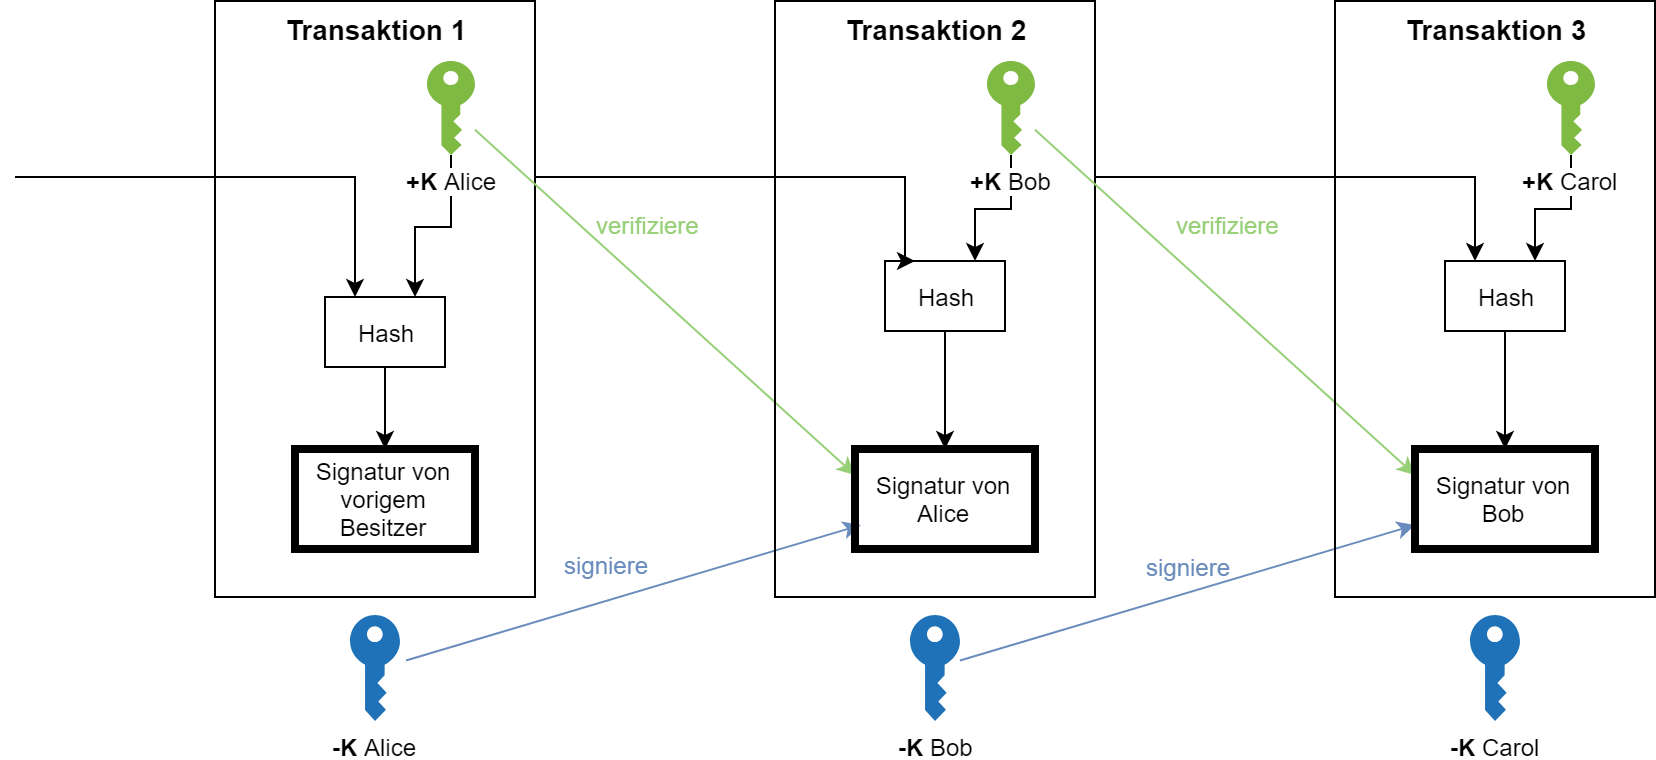
\includegraphics[width=0.9\textwidth]{graphics/transaction.png}
	    	\caption{Kette digitaler Signaturen}
	    	\label{fig:txio}
	    \end{figure}
    
	    Wie in \fref{fig:txio} dargestellt, werden Assets von einem Versender zu einem Empfänger transferiert, in dem der Sender einen Hash der vorigen Transaktion und den öffentlichen Schlüssel des Empfängers mit seinem eigenen privaten Schlüssel digital signiert und diese Hash dann am Ende des Assets anfügt.
	    Transaktionen können zudem mehrere Ein- und Ausgaben haben\cite{Nakamoto2008}.
	    Der Empfänger, sowie alle Teilnehmer des Netzwerkes können den Besitz des Assets über die Kette der digitalen Signaturen zurückverfolgen\cite{Nakamoto2008}.
    
    
    \begin{figure}[H]
        \missingfigure[figheight=4cm]{Bild mit Transaktion}
    \end{figure}
    
    \subsubsection{Sicherheit}
    \label{sec:blockchain_security}
    Byzantine Fault Tolerance
    
    \subsubsection{Identity Management}
    \label{sec:blockchain_identitymgmnt}
    \subsubsection{Self-Sovereign Identitity}
    \label{sec:blockchain_sovreign}

\subsection{Internet of Things}
    \subsubsection{Sicherheit}
    \subsubsection{Protokolle (BLE, Z-WAVE)}
    \subsubsection{Smart Homes}

\subsection{Smart Locks}
    \subsubsection{Häufig vorgefundene Gemeinsamkeiten}




    \section{Vorgehen}

\subsection{Analyse}


\subsection{Ableiten der Anforderungen an den Prototypen}

    \begin{itemize}
        \item Self-Sovereign Identitiy
        \item Decentralized Identifiers
    \end{itemize}
    \subsection{Prototyp}
\subsection{Auswahl des Frameworks}



\subsubsection{Architektur und Funktionsweise}
    Enstprechend dem Kapitel mit dem Stand der Wissenschaft wurden die Konzepte im Framework umgesetzt.
    
    \section{Evaluation des Prototypen}
\label{sec:evaluation}
    \section{Schluss}
\subsection{Ausblick}
	Ideen zur Erweiterung des Prototypen
	\begin{itemize}
		\item Self-Sovereign Identitiy
		\item Decentralized Identifiers
	\end{itemize}
    \nocite{*}

	%!!!!!!!!!!!!!!!!!!!!!!!!BIS HIER ARBEITEN!!!!!!!!!!!!!!!!!!!!!!!!
	%########################################################################################################
	
	
\newpage	
\printbibliography[title=Literaturverzeichnis]
\end{document}